
\newcommand{\contextSubSectionOneTitle}{A Broad Context:\\From the IoT to Large-scale Robotic Ensembles}

%A Broad Context: From the IoT to
\subsection{Large-scale Robotic Ensembles}

\newcommand{\iotversion}[1]{fig/Iot/#1}

\newcommand{\iotslide}[2]{
\noLogo{
\begin{frame} \frametitle{\contextSubSectionOneTitle{}}
	
	\begin{center}
		\begin{columns}[c]
			\begin{column}{.33\textwidth}
				\vspace{1cm}
				\begin{center}
					\includegraphics[width=\linewidth]{\iotversion{#1}}
				\end{center}
			\end{column}
			\begin{column}{.66\textwidth}
					#2
			\end{column}
		\end{columns}
	\end{center}
\end{frame}
}
}

\noLogo{
	\begin{frame} \frametitle{Large-scale Robotic Ensembles}
	
	\vspace{-0.5cm}
	\begin{center}
		\begin{columns}[c]
			\begin{column}{.25\textwidth}
				\centering
				\includegraphics[width=\linewidth]{\iotversion{iot-oval-lre}}
			\end{column}
			\begin{column}{.75\textwidth}
				
					{
					\setbeamercovered{invisible}
					%Large-scale robotic ensembles:
					\begin{itemize}
						\item Modular robotics, swarm robotics, distributed MEMS, robotic materials
						\item Macro-scale: reconfigurable IoRT objects
						\item Micro-scale: self-organized ensembles 
						\begin{itemize}
							\item up to $10^6$ units
							\item small and resource-constrained (energy, memory, computation) units 
						\end{itemize}
						\item Advantages: versatility, robustness, cheaper
					\end{itemize}
					}	
			\end{column}
		\end{columns}
	
		\begin{columns}[c]
			\begin{column}{.5\textwidth}
				\centering
				\href{run:videos/3-smartblocks.avi?autostart&loop}{\adjincludegraphics[width=0.9\linewidth,valign=c]{videos/3-smartblocks.jpg}}\\
				Conveying Surface\\Smart Blocks project (FEMTO-ST)
			\end{column}
			\begin{column}{.5\textwidth}
				\centering
				\href{run:videos/3-claytronics.mp4?autostart&loop}{\adjincludegraphics[width=0.9\linewidth,valign=c]{videos/3-claytronics.jpg}}\\
				Programmable Matter\\Claytronics project (CMU)
			\end{column}
		\end{columns}
		
	\end{center}
	
\end{frame}
}


\subsection{An Inter-Disciplinary Domain}

%A Caricatural Vision
\definecolor{thisThesisColor}{RGB}{255,204,0} 
\begin{frame} \frametitle{An Inter-Disciplinary Domain}

\begin{center}
\begin{columns}[c]
	\begin{column}{.6\textwidth}
		\centering
		\only<1>{
		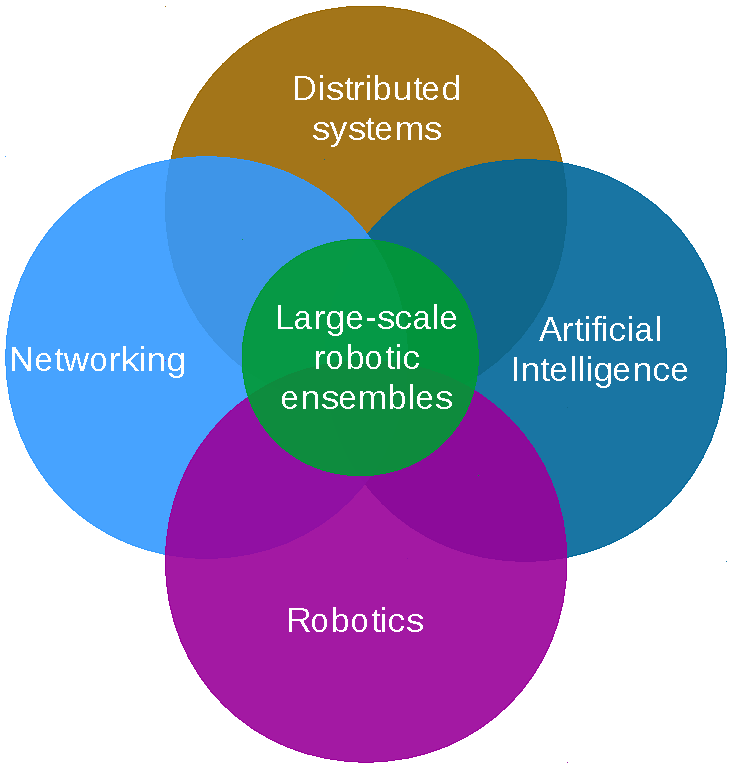
\includegraphics[width=\textwidth]{fig/domains/domains-not-positioned}
		}
		\only<2>{
		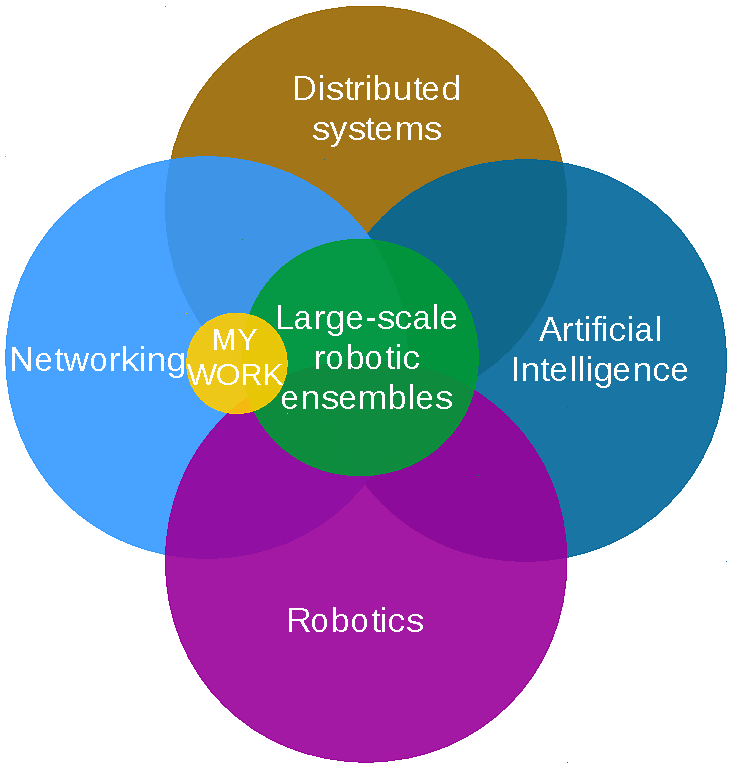
\includegraphics[width=\textwidth]{fig/domains/domains}
		}
	\end{column}
	\begin{column}{.4\textwidth}		
		Challenges:
		\begin{itemize}
			\item Hardware: Fabrication
			\item \tikzmark{start}Algorithmic: Distributed \tikzmark{end} coordination
		\end{itemize}
	\end{column}
\end{columns}
\end{center}

\begin{tikzpicture}[remember picture,overlay]
\draw<2>[draw, line width=2pt,thisThesisColor,label={[xshift=1.0cm, yshift=-0.15cm,align=center]\textcolor{thisThesisColor}{My work}}] (9.92,3.5) ellipse (2.5 and 0.6);
\node<2> at ($(9.92,2.6)$) {\textcolor{thisThesisColor}{my work}};
%
%\node<2>[draw,line width=2pt,cyan,circle,fit={(pic cs:start) (pic cs:end)}] {};
\end{tikzpicture}

\end{frame}